\section{Methodology}

\subsection{Control Objective}

Reward mashes throughput, latency-shaped terms, a decentralization proxy, and distance to a moving target:
\[
\begin{aligned}
r ={}& w_1 \cdot \text{throughput} + w_2 \cdot \text{latency}(d) \\
&+ w_3 \cdot \text{decentralization} - \lambda |d - d_t|.
\end{aligned}
\]
Shield always sees actions after clipping.

\subsection{Policy Family}

Controllers span random, hand-tuned heuristics, vanilla PPO-family runs, and the robust gated recipe. PPO stays clipped \cite{schulman2017ppo}; our robust branch subtracts rolling reward variance:
\[
\tilde r_t = r_t - \lambda_{\mathrm{risk}}\,\mathrm{Var}(r_{t-k:t}).
\]

\subsection{Shield Logic (Executable Rule)}

Shield code is deterministic, state-aware, and boring on purpose---box constraints plus a per-step slew cap before anything executes:
\[
a^{\mathrm{exec}}_t=\mathrm{clip}(a_t, a_{\min}, a_{\max}),
\]
\[
\Delta a_t=\mathrm{clip}(a^{\mathrm{exec}}_t-a_{t-1},-\delta_{\max},\delta_{\max}).
\]
Still unsafe on a predicate (delay projection, partition threshold, etc.)? Swap to heuristic $a_t^{\mathrm{heur}}$ and re-run the checks. Code-level sketch:
\begin{itemize}
    \item If \texttt{hard\_safe(state, action)} is false, clamp action by bounds and max delta.
    \item Re-check safety; if still false, switch to \texttt{heuristic\_action(state)}.
    \item Return the validated action.
\end{itemize}

For explicit auditability, shield execution is summarized below:
\begin{enumerate}
    \item Input $(s_t, a_t, a_{t-1})$.
    \item Set $a\leftarrow\mathrm{clip}(a_t,a_{\min},a_{\max})$.
    \item Set $a\leftarrow a_{t-1}+\mathrm{clip}(a-a_{t-1},-\delta_{\max},\delta_{\max})$.
    \item If $\mathrm{hard\_safe}(s_t,a)$, return $a$.
    \item Set $a_h\leftarrow\mathrm{heuristic\_action}(s_t)$.
    \item Set $a_h\leftarrow\mathrm{clip}(a_h,a_{\min},a_{\max})$.
    \item Set $a_h\leftarrow a_{t-1}+\mathrm{clip}(a_h-a_{t-1},-\delta_{\max},\delta_{\max})$.
    \item If $\mathrm{hard\_safe}(s_t,a_h)$, return $a_h$.
    \item Otherwise, return $\mathrm{emergency\_safe\_action}(s_t)$.
\end{enumerate}

\subsection{Quantum-Inspired Uncertainty Gate}

Front-end is a six-qubit variational sketch: angle embed, entangle, re-upload data, read Pauli-$Z$ for mean/scale-ish scalars. Uncertainty comes from shaking weights, not from mysticism:
\[
\begin{aligned}
u_q(x) &= \operatorname{Var}\left(\{\mu_{\theta+\epsilon_k}(x)\}_{k=1}^{K}\right), \\
\epsilon_k &\sim \mathcal{N}(0,0.01I),\quad K=10.
\end{aligned}
\]
The routing rule is
\[
a_t=
\begin{cases}
a_t^{\mathrm{heur}}, & u_q(x_t)>\tau_q,\\
a_t^{\mathrm{policy}}, & u_q(x_t)\le\tau_q.
\end{cases}
\]

\subsection{Engineering Trade-offs in Uncertainty Design}

Offline pretty plots were not the bottleneck---serving cost was. Ensembles mean N forwards per step and N copies in RAM; perturbation keeps one net and jitters $\theta$ at inference, which is easier to colocate with a controller loop.

In our head-to-head grid the perturbation readout bought precision at fixed trigger budget versus MC-dropout and a small ensemble baseline without torching recall, so tuning targeted ``routing good enough at 10\% fire rate'' instead of chasing a single scalar uncertainty KPI.

\begin{figure}[H]
\centering
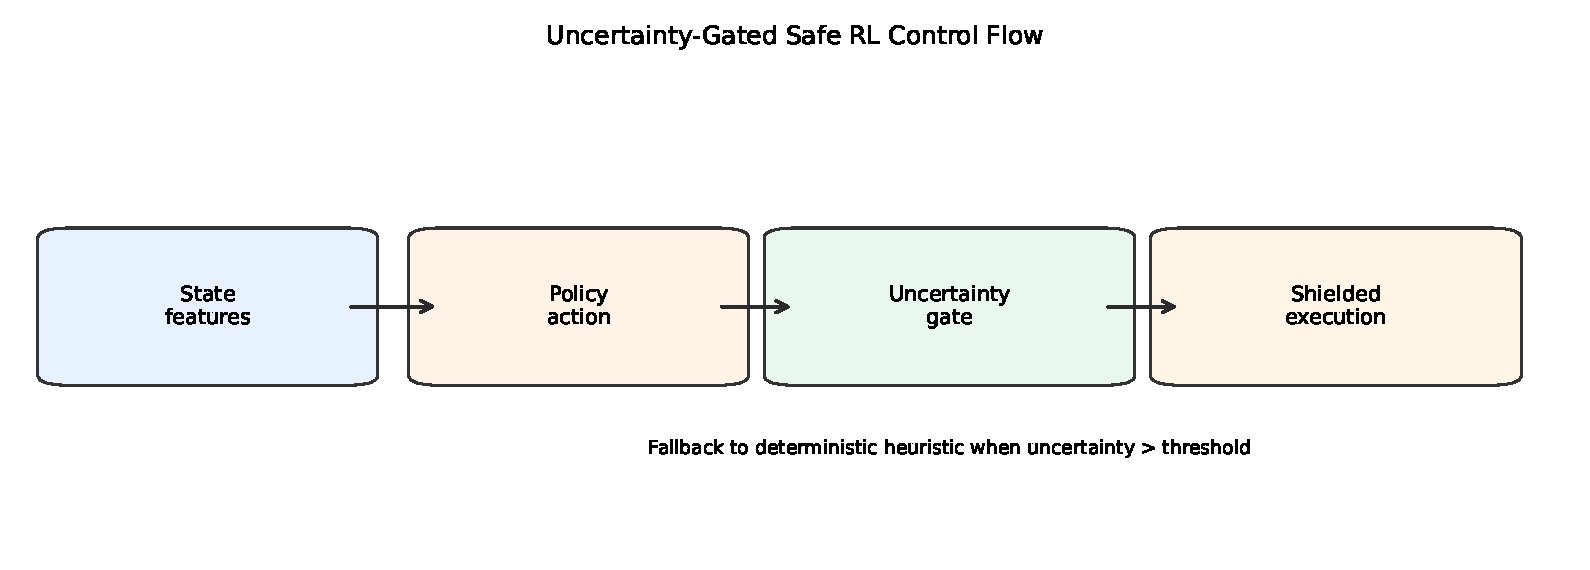
\includegraphics[width=0.88\linewidth]{figures/robust_policy_flow.pdf}
\caption{Fallback path: perturbation uncertainty $\rightarrow$ gate $\rightarrow$ shielded execution.}
\label{fig:robust-flow}
\end{figure}

\subsection{Why the Compact Estimator Compresses Well Here}

Classical simulation only; quantum throughput is irrelevant. Governance vectors in our build jam delay, congestion, attack pressure, and nasty cross-terms. Entangling layers mix multiplicatively on the cheap; re-uploading lets the same wires bend across time. Net effect: fewer weights than a fat MLP for the surface we needed. Compression only popped once gate+shield were live---without them the head trained on regimes it never had to stabilize.

\subsection{Adversarial and Ablation Design}

Scaled workload throws bursts, noisy delay, attack ramps, and regime hops. Seven toggles:
\begin{itemize}
    \item full system (quantum gate + shield + robust policy),
    \item no quantum gate,
    \item no shield,
    \item no fallback,
    \item classical PPO,
    \item Heuristic controller,
    \item random.
\end{itemize}
The stress-aware reward is
\[
\begin{aligned}
r_t^{\text{adv}} ={}& \alpha\,\text{throughput}_t - \beta\,\text{delay}_t - \gamma\,\text{attack}_t \\
&- \eta\,\text{fork}_t - \lambda |d_t-d^\star|.
\end{aligned}
\]

\subsection{Evaluation}

Scalars first: reward, violations, target MAE, fallback counters, a latency stand-in. Whenever two PPO-family rows get compared we bolt on bootstraps, permutation tests, and Cohen's $d$ so a single seed draw cannot ghost-write the conclusion \cite{efron1994introduction,good2005permutation}.